\section{Resultados y análisis}

\subsection*{Red hogareña}
\subsubsection*{Resultados fuente S1}
\begin{figure}[H]
  \centering
  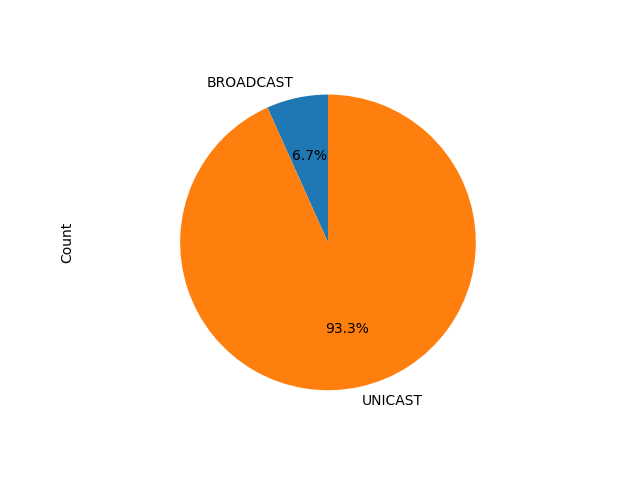
\includegraphics[width=8.5cm]{figs/broadcast_proportion_hogar_ethernet_S1_output.png}
  \caption{\normalfont Proporción de paquetes unicast/broadcast en la captura}
\end{figure}

\begin{figure}[H]
  \centering
  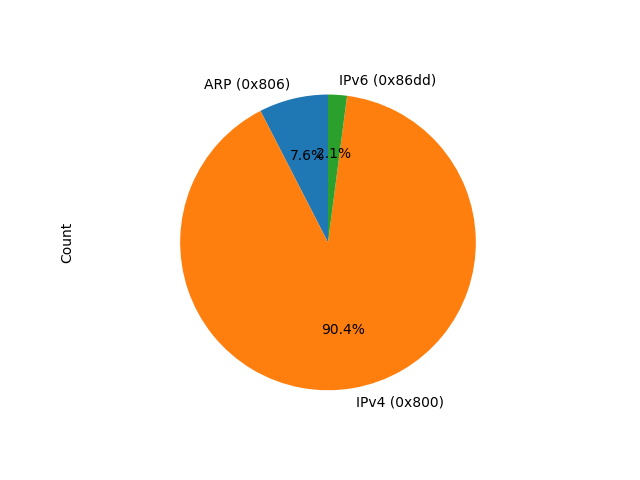
\includegraphics[width=8.5cm]{figs/protocols_proportion_hogar_ethernet_S1_output.png}
  \caption{\normalfont Proporción de protocolos en la captura}
\end{figure}

\begin{figure}[H]
  \centering
  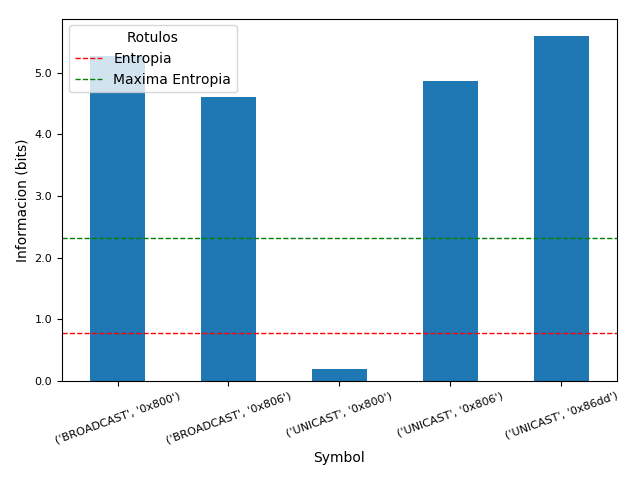
\includegraphics[width=8.5cm]{figs/information_hogar_ethernet_S1_output.png}
  \caption{\normalfont Información de los símbolos de la fuente S1, notando la entropía de la fuente, y la máxima entropía posible si la fuente fuera equiprobable.}
\end{figure}

\subsubsection*{Resultados fuente S2}

A partir de los paquetes que se intercambian en distintas redes vemos los grafos subyacentes a las mismas. En estos cada vertice representa una IP local y cada arista va del origen al destino de un paquete who-has del protocolo ARP.

\begin{figure}[H]
  \centering
  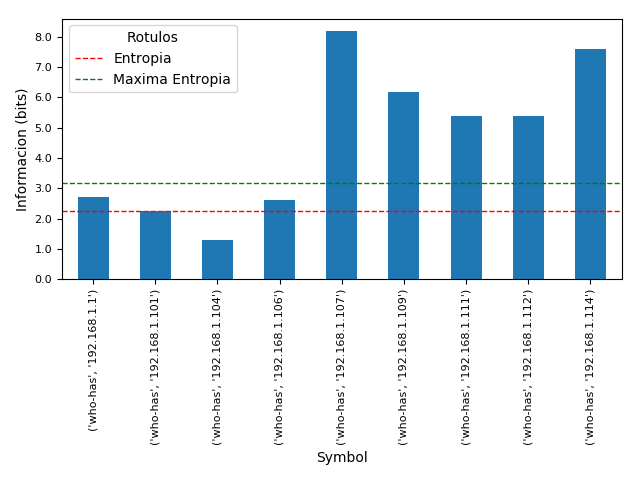
\includegraphics[width=8.5cm]{figs/information_hogar_ethernet_S2_output.png}
  \caption{\normalfont Información de los símbolos de la fuente S2, notando la entropía de la fuente, y la máxima entropía posible si la fuente fuera equiprobable.}
\end{figure}

En este grafo los dos nodos con mayor grado son 192.168.1.1 con grado 7 y 192.168.1.112

\begin{figure}[H]
 \centering
	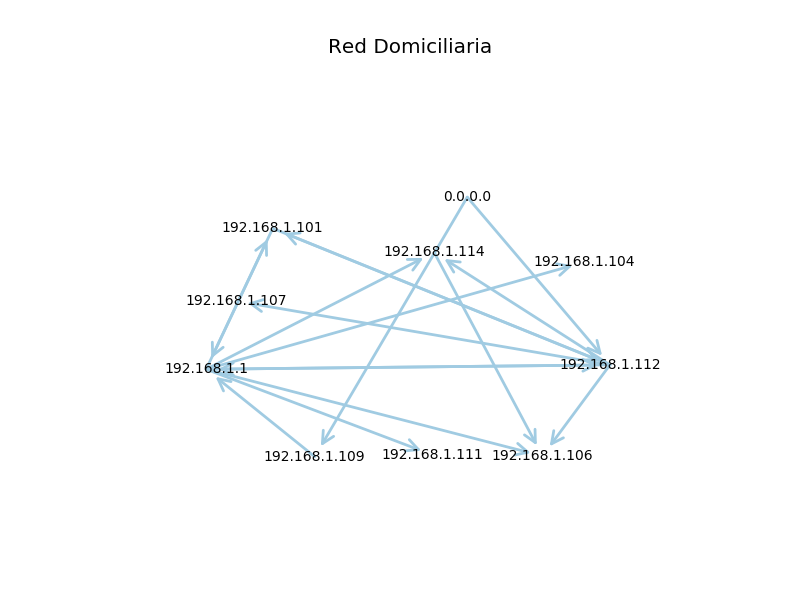
\includegraphics[width=8.5cm]{figs/red_domiciliaria.png}
	\caption{Grafo resultante de la red ethernet de una red domiciliaria durante la noche de un día de semana.}
	\label{fig:starbucks-grafo}
\end{figure}

Este grafo tiene solo dos nodos de los cuales el único que recibe paquetes es el nodo 172.19.96.1

\subsection*{Red laboratorios}

\subsubsection*{Resultados fuente S1}
\begin{figure}[H]
  \centering
  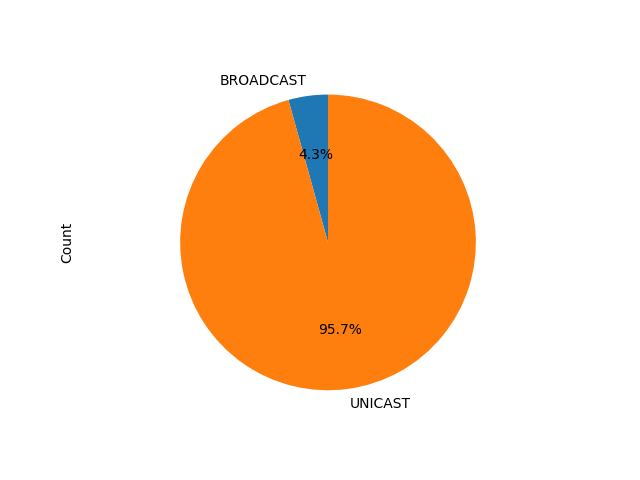
\includegraphics[width=8.5cm]{figs/broadcast_proportion_labo6_2018_04_18_S1_output.png}
  \caption{\normalfont Proporción de paquetes unicast/broadcast en la captura}
\end{figure}

\begin{figure}[H]
  \centering
  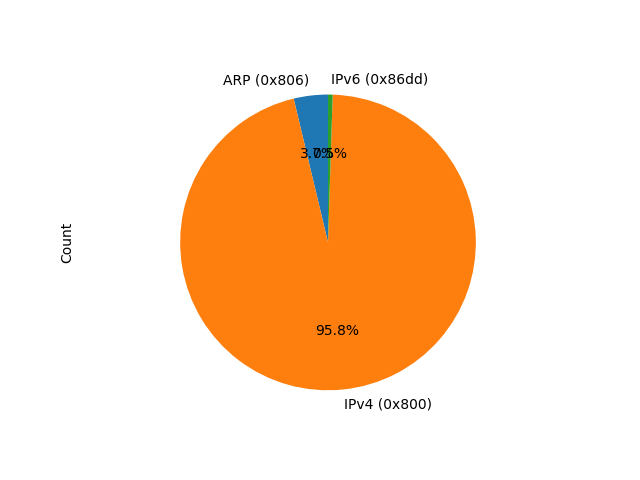
\includegraphics[width=8.5cm]{figs/protocols_proportion_labo6_2018_04_18_S1_output.png}
  \caption{\normalfont Proporción de protocolos en la captura}
\end{figure}

\begin{figure}[H]
  \centering
  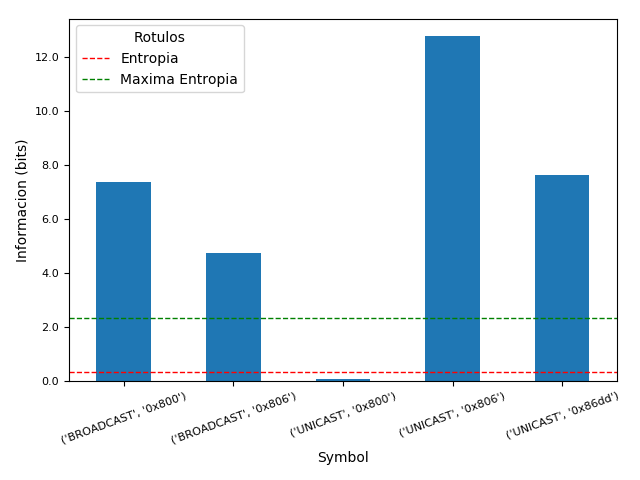
\includegraphics[width=8.5cm]{figs/information_labo6_2018_04_18_S1_output.png}
  \caption{\normalfont Información de los símbolos de la fuente S1, notando la entropía de la fuente, y la máxima entropía posible si la fuente fuera equiprobable.}
\end{figure}

\subsubsection*{Resultados fuente S2}

\begin{figure}[H]
  \centering
  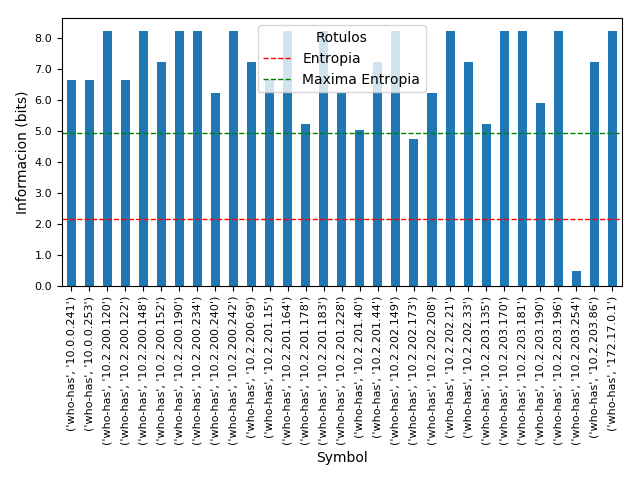
\includegraphics[width=8.5cm]{figs/information_labo6_2018_04_18_S2_output.png}
  \caption{\normalfont Información de los símbolos de la fuente S2, notando la entropía de la fuente, y la máxima entropía posible si la fuente fuera equiprobable.}
\end{figure}

Este grafo es mucho mas grande que los anteriores y cuenta con un nodo de máximo grado el cual es el 10.2.203.254.

\begin{figure}[H]
 \centering
	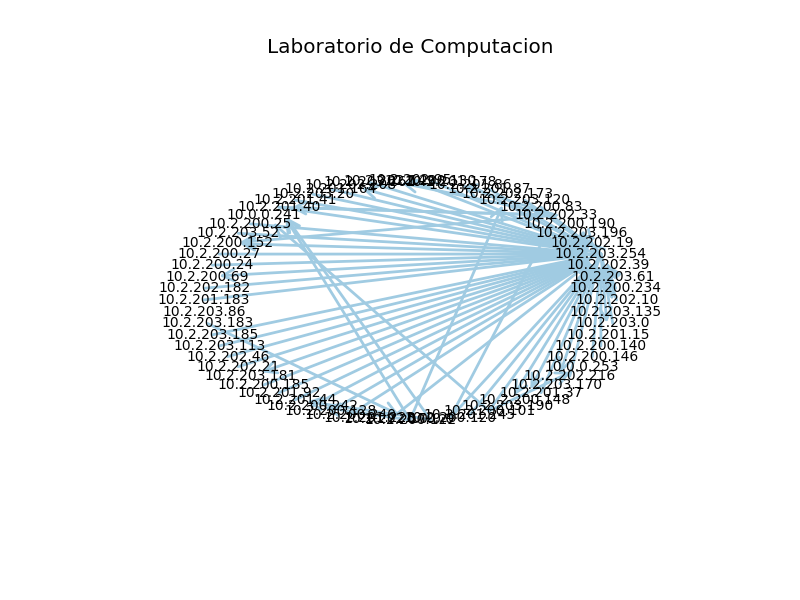
\includegraphics[width=8.5cm]{figs/dc.png}
	\caption{Grafo resultante de la red wifi del laboratorio de computación de la facultad a las 18 PM de un miércoles.}
	\label{fig:dc-grafo}
\end{figure}

\subsection*{Red Starbucks}
\subsubsection*{Resultados fuente S1}
\begin{figure}[H]
  \centering
  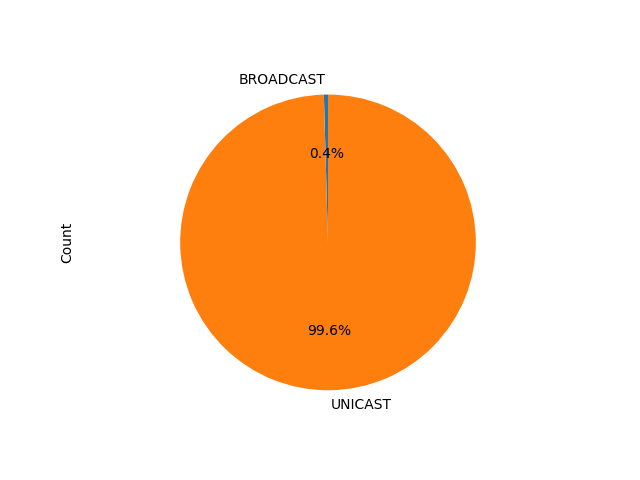
\includegraphics[width=8.5cm]{figs/broadcast_proportion_starbucks_S1_output.png}
  \caption{\normalfont Proporción de paquetes unicast/broadcast en la captura}
\end{figure}

\begin{figure}[H]
  \centering
  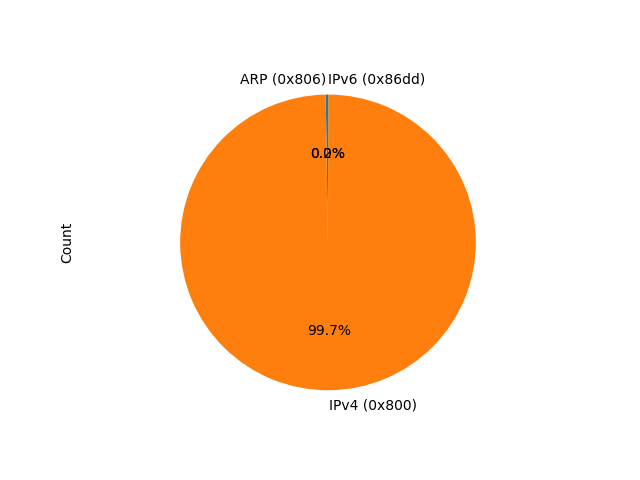
\includegraphics[width=8.5cm]{figs/protocols_proportion_starbucks_S1_output.png}
  \caption{\normalfont Proporción de protocolos en la captura}
\end{figure}

\begin{figure}[H]
  \centering
  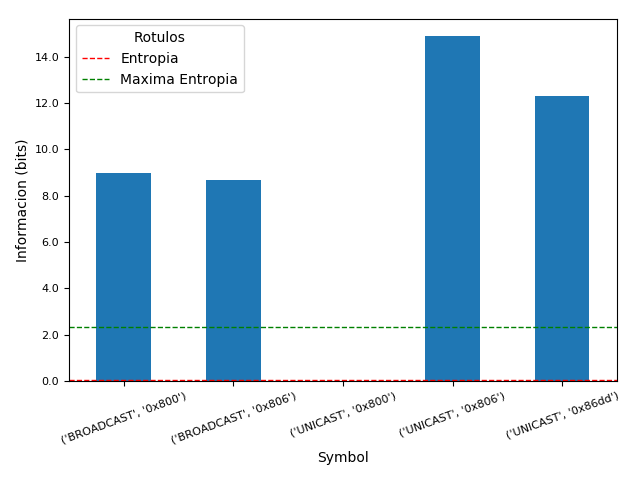
\includegraphics[width=8.5cm]{figs/information_starbucks_S1_output.png}
  \caption{\normalfont Información de los símbolos de la fuente S1, notando la entropía de la fuente, y la máxima entropía posible si la fuente fuera equiprobable.}
\end{figure}

\subsubsection*{Resultados fuente S2}

Este grafo tiene solo dos nodos de los cuales el unico que recibe paquetes es el nodo 172.19.96.1

\begin{figure}[H]
 \centering
	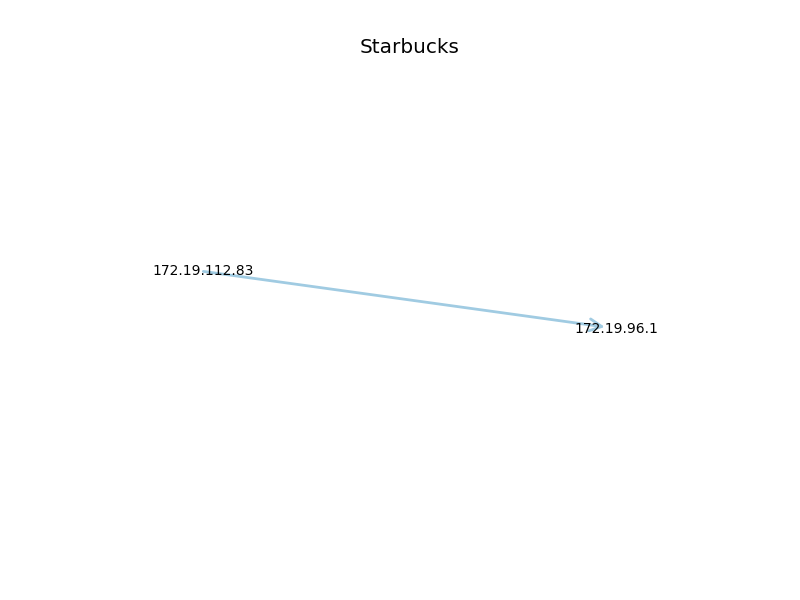
\includegraphics[width=8.5cm]{figs/starbucks.png}
	\caption{Grafo resultante de la red wifi de una red pública en un starbucks durante la tarde de un día de semana.}
	\label{fig:domicilio-grafo}
\end{figure}
